\subsubsection{Squirmerの運動方程式}
\label{sec:equation_of_motion}
    \begin{align}
        \dot{\boldsymbol{R}_i} &= \boldsymbol{V}_i \\
        M_\mathrm{p} \dot{\boldsymbol{V}_i} &= \boldsymbol{F}^\mathrm{H}_i \\
        \boldsymbol{I}_\mathrm{p} \cdot \dot{\boldsymbol{\Omega}_i} &=
            \boldsymbol{N}^\mathrm{H}_i + \boldsymbol{N}^\mathrm{b.h.}_i
    \end{align}

\noindent
ここで,$\boldsymbol{F}^\mathrm{H}_i$は流体から受ける力,
$\boldsymbol{N}^\mathrm{H}_i$は流体から受けるトルク,
$\boldsymbol{N}^\mathrm{b.h.}_i$はbottom heavy性によるトルクである.
$M_\mathrm{p}$は粒子の質量,
$\boldsymbol{I}_i$は慣性モーメント,
$\dot{\boldsymbol{R}_i}$は粒子の位置,
$\boldsymbol{V}_i$は粒子の速度,
$\dot{\boldsymbol{\Omega}_i}$は粒子の角速度である.
Fig.\ref{fig:bottom_heaviness}のように,
球の中心と粒子の重心がずれている,
bottom heavy性を有するsquirmerについて,
その性質に起因するトルクは式\eqref{eq:bottom_heavy_torque}で計算される\cite{dilute_squirmer}.

    \begin{equation}
        \boldsymbol{N}^\mathrm{b.h.} = \frac{4}{3} \pi a^3 \rho h \boldsymbol{\hat{e}} \times \boldsymbol{g}
        \label{eq:bottom_heavy_torque}
    \end{equation}

\noindent
ここで,$a$は粒子の半径,
$\rho$は粒子の密度,
$h$は球の中心と粒子の重心との距離,
$\boldsymbol{\hat{e}}$は粒子の方向ベクトル,
$\boldsymbol{g}$は重力ベクトルである.

    \begin{figure}[htbp]
        \centering
        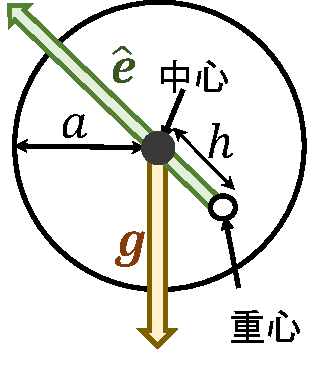
\includegraphics[scale=0.8]{/Users/taiga/Projects/lab/thesis/components/chapter2/figs/bottom_heavy.pdf}
        \caption{bottom heavy性を有するsquirmer}
        \label{fig:bottom_heaviness}
    \end{figure}
